\documentclass[smaller,professionalfonts]{beamer}
\usepackage{fontspec,unicode-math}
\usepackage{lipsum, lmodern}
\usepackage{bncc}
\usepackage{polyglossia}
\setdefaultlanguage[%
   variant=american
]{english}

\usetheme[widescreen]{PraterStreet} % or Median, or Metro, or PraterStreet, or Milano

\setromanfont{Abyssinica SIL}
\setsansfont{Abyssinica SIL}
\setmonofont[Color={0019D4}]{Abyssinica SIL}

\title{Machado de Assis}
\author{O pai contra mãe}
\institute{Thema: Contos}
\date{}

\begin{document}

%Abertura
\frame{\maketitle}


%Obra/Autor
\begin{frame}[plain]{Machado de Assis}
\centering\LARGE\textbf{O autor e a obra}\\\bigskip
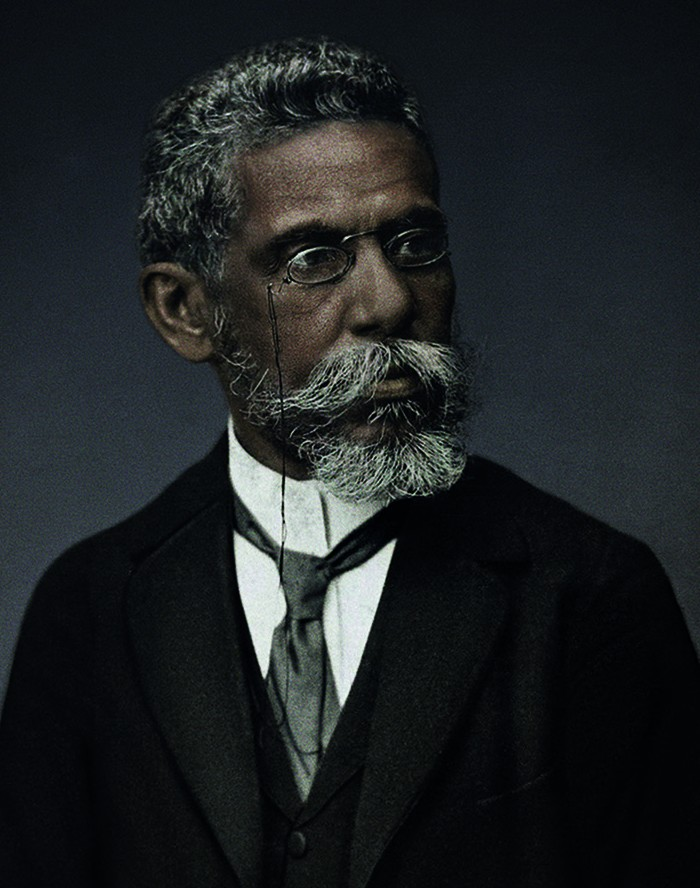
\includegraphics[scale=0.15]{author}
\end{frame}

%Motivação
\begin{frame}[plain]{Por que ler?}
\begin{block}{Tema}
Diálogos com a sociologia e com a antropologia
\end{block}
\bigskip
\begin{columns}
\column{0.5\textwidth}
Mussum Ipsum, cacilds vidis litro abertis. Quem manda na minha terra sou euzis! Tá deprimidis, eu conheço uma cachacis que pode alegrar sua vidis. Nullam volutpat risus nec leo commodo, ut interdum diam laoreet. Sed non consequat odio. Interagi no mé, cursus quis, vehicula ac nisi.
\column{0.5\textwidth}
Mussum Ipsum, cacilds vidis litro abertis. Quem manda na minha terra sou euzis! Tá deprimidis, eu conheço uma cachacis que pode alegrar sua vidis. Nullam volutpat risus nec leo commodo, ut interdum diam laoreet. Sed non consequat odio. Interagi no mé, cursus quis, vehicula ac nisi.
\end{columns}

\end{frame}

%Gên./Mov.
\begin{frame}{Teste de BNCC}
\BNCC{EM13LGG302}
\end{frame}

%Habilidades (1)
\begin{frame}
\frametitle{Quadro de habilidades}
\begin{block}{EM13LGG302}
Compreender e posicionar-se criticamente diante de diversas visões de mundo presentes nos discursos em diferentes linguagens,/ levando em conta seus contextos de produção e de circulação
\end{block}
\begin{block}{EM13LP45}
Compartilhar sentidos construídos na leitura/escuta de textos literários,/ percebendo diferenças e eventuais tensões entre as formas pessoais e coletivas de apreensão desses textos,/ para exercitar o diálogo cultural e aguçar a perspectiva crítica. 
\end{block}
\end{frame}

%Encerramento
\begin{frame}
\frametitle{}
\centering\Large\textbf{Obrigado}
\end{frame}


% \begin{frame}
% \frametitle{Using Columns}
% \begin{columns}
% \column{0.5\textwidth}
% Mussum Ipsum, cacilds vidis litro abertis. Quem manda na minha terra sou euzis! Tá deprimidis, eu conheço uma cachacis que pode alegrar sua vidis. Nullam volutpat risus nec leo commodo, ut interdum diam laoreet. Sed non consequat odio. Interagi no mé, cursus quis, vehicula ac nisi.
% \column{0.5\textwidth}
% Mussum Ipsum, cacilds vidis litro abertis. Quem manda na minha terra sou euzis! Tá deprimidis, eu conheço uma cachacis que pode alegrar sua vidis. Nullam volutpat risus nec leo commodo, ut interdum diam laoreet. Sed non consequat odio. Interagi no mé, cursus quis, vehicula ac nisi.
% \end{columns}
% \end{frame}

\end{document}
